\documentclass[aspectratio=169]{beamer}

\usetheme{Madrid}
\usecolortheme{default}

\title[Typescript]{Typescript}
\subtitle{И не Javascript}
\author{Кормышев Егор ИСиП-301}
\date{\today}

\usepackage[russian]{babel}
\usepackage{minted}
\usepackage{graphicx}

\begin{document}

\frame{\titlepage}

% Frame 1: Introduction

\begin{frame}

  \frametitle{Вступление}
  \begin{center}
    \large{Что такое TypeScript?} \\
  \end{center}
  \bigskip
  \bigskip

  \normalsize\textcolor{blue}{Typescript} - Это язык программирования, изначально \\ созданный для упрощения жизни javascript-программистов
  
\end{frame}

\begin{frame}

  \begin{center}    
    Он добавляет к javascript статическую типизацию: 
    
    \bigskip

    \alert{\large{Javascript}} \\
    \bigskip
    \normalsize 1 + "яблоко" \  = "1яблоко"
    \bigskip

    \textcolor{blue}{\large{Typescript}} \\
    \bigskip
    \normalsize 1 + "яблоко" \  = \alert{Error}
    
  \end{center}
  
\end{frame}

\begin{frame}[fragile]
  И добавляет более понятные ошибки

  \bigskip
  
  \small{Например:}

  \begin{block}{Код}
    \begin{minted}{typescript}    
      function add(a:number, b:number): number {
        return a + b;
      }

      add(1, "яблоко");

    \end{minted}
  \end{block}

  \begin{alertblock}{Ошибка}
    \texttt{
      sample.ts:5:8 - error TS2345: Argument of type 'string' is not assignable to parameter of type 'number'. (тип "число" нельзя привести к типу "строка")
    }
  \end{alertblock}
  
\end{frame}

% variables with types

\begin{frame}[fragile]

  \frametitle{Типизация переменных}

  \begin{minted}{typescript}
    let name:string = "Alex"; 
  \end{minted}

  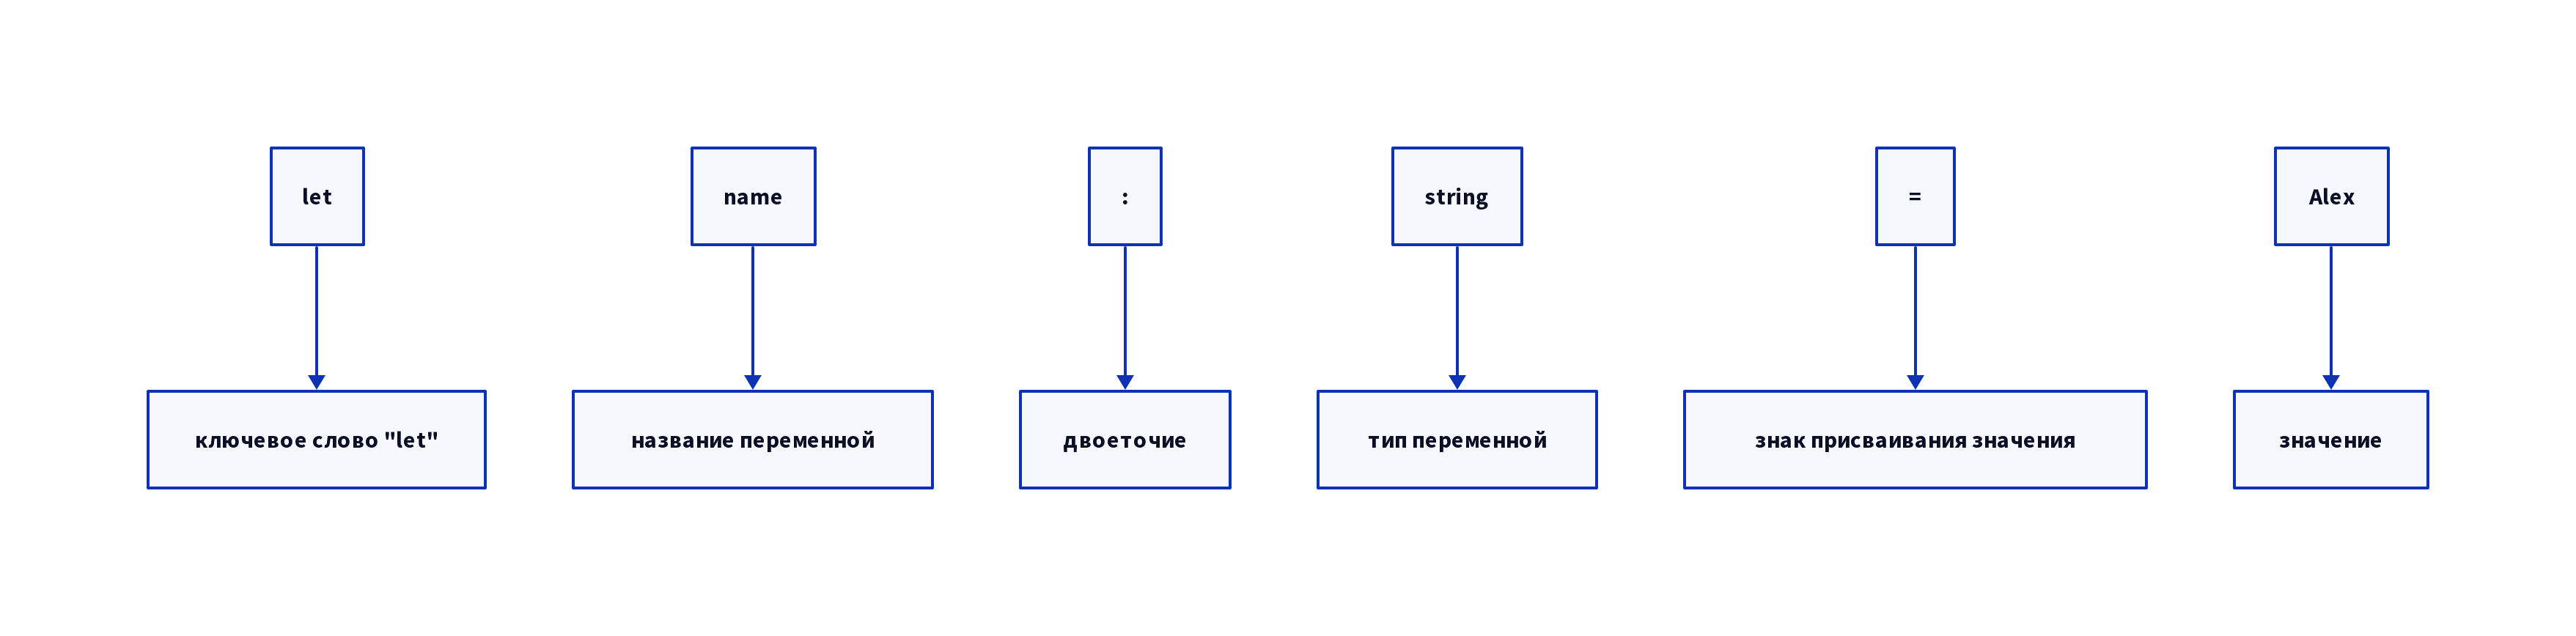
\includegraphics[width=\textwidth]{assets/description.png}
  
\end{frame}

% basic types

\begin{frame}

  \frametitle{Базовые типы}
  \begin{itemize}
  \item \texttt{string} - строка - "qwerty", 'hello world' \\
  \item \texttt{number} - число (целое и дробное) - 3, 1.5 \\
  \item \texttt{boolean} - логическое - true, false \\
  \item \texttt{null} - ничего (пустая переменная) - null \\
  \item \texttt{undefined} - неопределенное значение (значение может не существовать) - undefined \\
  \item \texttt{object} - объект - {}, {name:string, age:number} \\
  \item \texttt{void} - функция ничего не возвращает \\
  \end{itemize}
  
\end{frame}


\begin{frame}[fragile]

  \frametitle{Типизация объектов}

  \begin{alertblock}{Пример объекта в js}
    \begin{minted}{javascript}
      let user = {
        name: "Alex",
        age: 25,
        isAdmin: false
      }
    \end{minted}
  \end{alertblock}

\end{frame}

\begin{frame}[fragile]

  \begin{block}{Типизированная версия}
    \begin{minted}{typescript}
      let user: {
        name: string,
        age: number,
        isAdmin:boolean
      } = {
        name: "Alex",
        age: 25,
        isAdmin: false
      }
    \end{minted}
  \end{block}
\end{frame}

% types on functions

\begin{frame}[fragile]

  \frametitle{Типизация функций}

  Чтобы типизировать функцию, нужно типизировать ее входные и выходные параметры

  \begin{block}{Пример}
    \begin{minted}{typescript}
      function isEven(num:number): boolean {
        if (num % 2 == 0) {
        return true
      } else {
        return false
      }
    }
  \end{minted}
\end{block}

В этом примере \texttt{number} - тип входного параметра \texttt{num}, а \texttt{boolean} - тип возвращаемого значения

\end{frame}

\begin{frame}[fragile]

  \frametitle{Типизация массивов}

  Есть 2 способа типизировать массив: \\
  Наиболее распространенный: \\ 
  \begin{minted}{typescript}
    let numbers: number[] = [1,2,3] 
  \end{minted}
  (Написать тип и поставить \texttt{[]} после него) \\

  И неиспользуемый: \\
  \begin{minted}{typescript}
    let numbers: Array<number> = [1,2,3] 
  \end{minted}
  (Написать тип \texttt{Array} и указать нужный тип как его generic \texttt{<>} после него)  
  
  
  
\end{frame}

\begin{frame}[fragile]

  \frametitle{Мультитипы}

  В \textcolor{blue}{Typescript} одно значение или параметр может иметь несколько типов. \\
  Для того чтобы указать это используется знак "побитовое или" (\texttt{|})

  \begin{block}{Пример}
    \begin{minted}{typescript}
      let stringOrNumber: string | number = 1;
    \end{minted}
    \begin{center}
      или
    \end{center}
    \begin{minted}{typescript}
      let stringOrNumber: string | number = "some string";
    \end{minted}

    \begin{center}
      При данной типизации оба значения верны
    \end{center}
    
  \end{block}
  
  
\end{frame}

\begin{frame}[fragile]

  \frametitle{Кастомные (Свои) типы}

  Для объявления типов используется cледующий синтаксис:

  \begin{minted}{typescript}
    type myBooleanString = string | boolean
  \end{minted}
  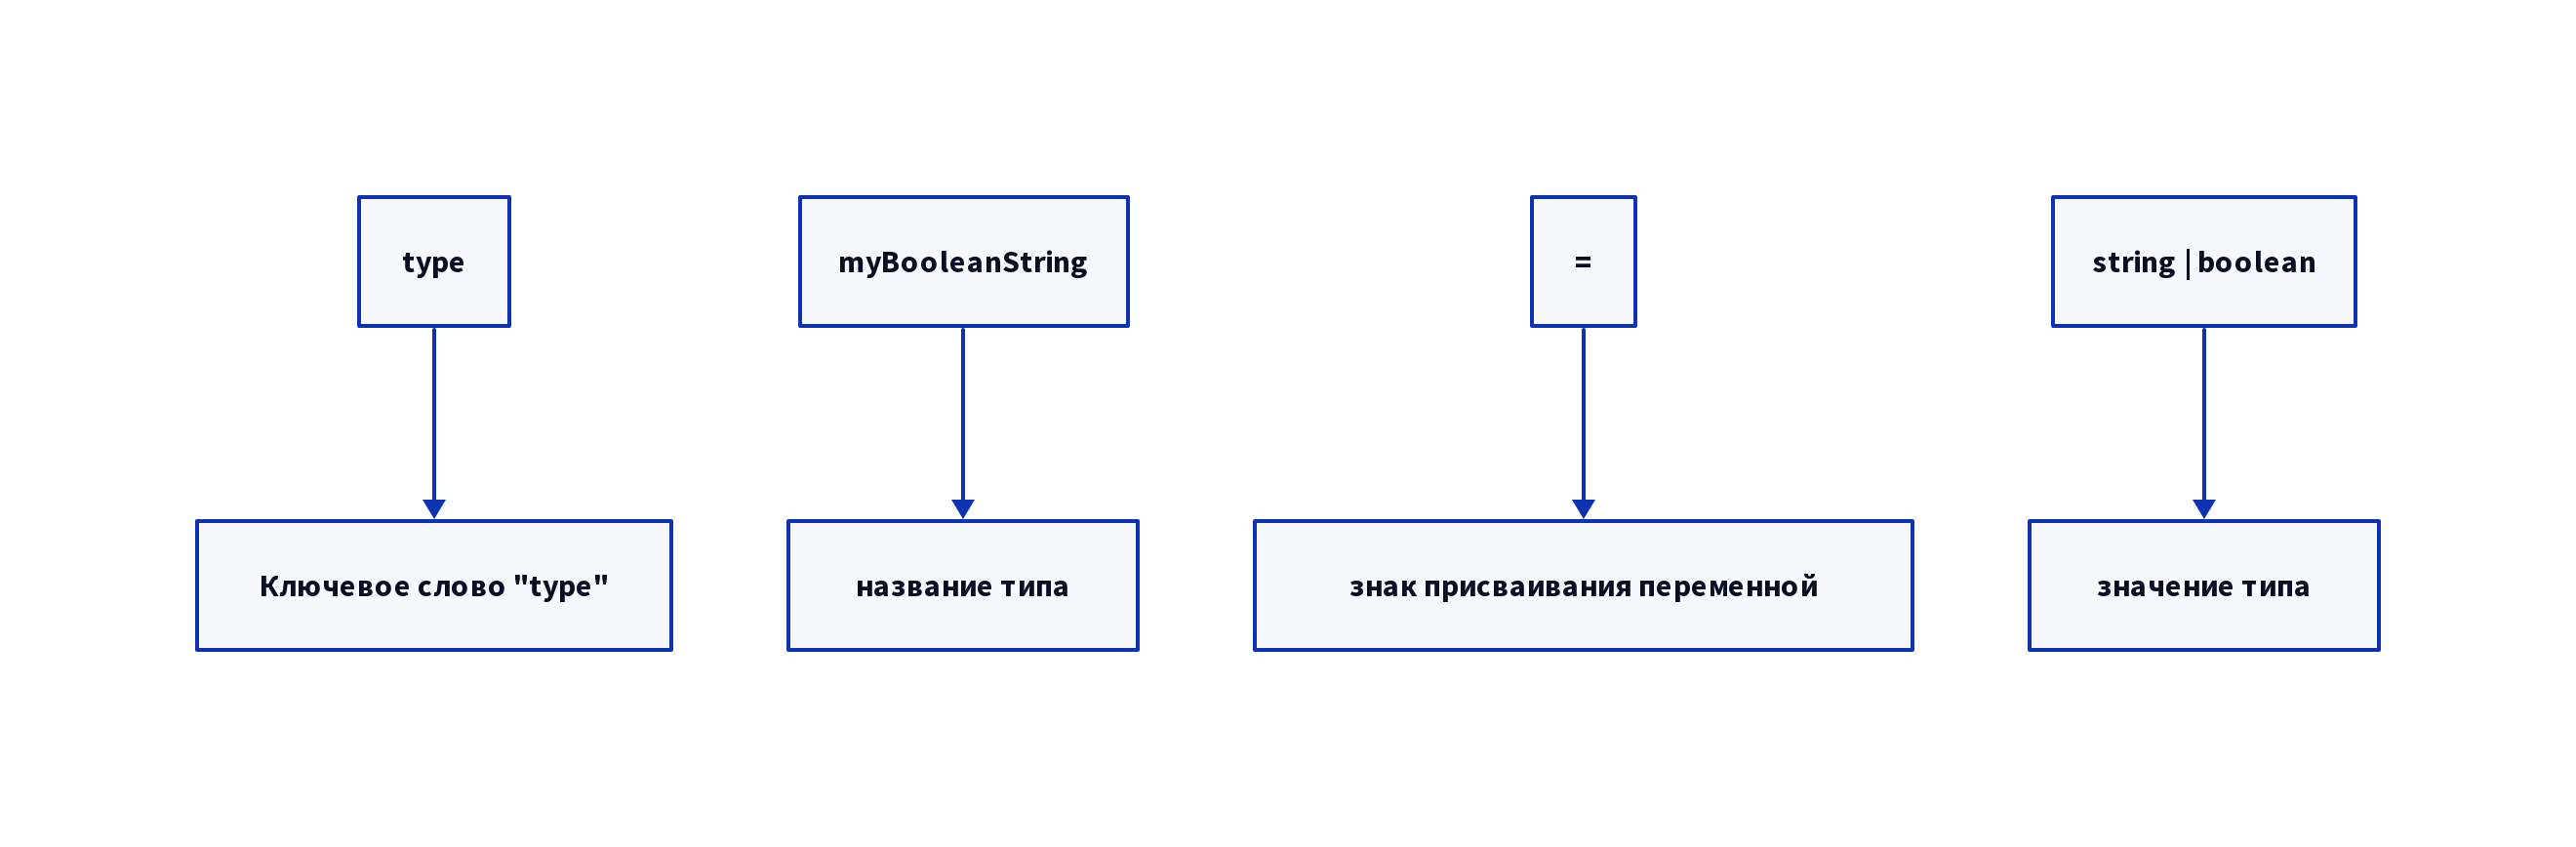
\includegraphics[width=\textwidth]{assets/custom_type.png}
\end{frame}

\begin{frame}[fragile]
  Теперь более сложный пример: свой тип объекта (правильная типизация объектов)
  
  \begin{block}{Пример}
    \begin{minted}{typescript}
      type User = {
        name: string,
        age: number,
        isAdmin: boolean
      }
    \end{minted}
    \begin{center}
      Таким образом, теперь для типизации объекта достаточно сделать следующее
    \end{center}
    \begin{minted}{typescript}
      let myUser: User = {...}
    \end{minted}
  \end{block}
  
\end{frame}


% Generics 

\begin{frame}[fragile]

  \frametitle{Generics. Обобщенные типы}

  Обобщенный тип означает что на его месте может быть любой тип
  
  Такой тип обозначается \texttt{<T>} (Вместо T может быть любая другая буква, но принято "T" т.к. type) \\

  \begin{block}{Пример написания Generic-функции}
    \begin{minted}{typescript}
      function gettype<T>(v: T): void {
        // орератор typeof возвращает тип переменной
        console.log(typeof v)
      }

      gettype(1)
      gettype(true)

    \end{minted}
    Результатом выполнения будет: \texttt{\newline number \newline boolean}
  \end{block}
  
\end{frame}

% Test

\begin{frame}

  \frametitle{Тест}

  \begin{enumerate}
  \item К какому типу принадлежат следующие значения: 4.56, 37, 23?
  \item Напишите 2 способа типизации массива логических значений
  \item Какой тип имеет функция в которой нет \texttt{return}? 
  \item Какой символ используется для обозначения мультитипа (несколько типов на одно значение)?
  \item как "отключить" типизацию?
  \end{enumerate}
  
\end{frame}

% Tasks

\begin{frame}[fragile,allowframebreaks]

  \frametitle{Задачи}

  \begin{enumerate}
  \item Типизировать функцию \texttt{pow} кторая принимает число и возвращает квадрат этого числа
  \item Дан объект \texttt{post}: \\
    \begin{minted}{javascript}
      let post = {
        id: 1,
        title: "Первый пост",
        content: "Какой-то пост о чем-то",
        stats: {
          likes: 3,
          reposts: 2
        }
      }
    \end{minted}
    Написать тип \texttt{Post} соответсвующий объекту

  \item Написать функию \texttt{isThree} которая принимает массив любого типа \texttt{<T>} и проверяет кол-во элементов в нем. \\
    Если их кол-во 3 или более - вернуть 3 элемент, иначе вернуть \texttt{null} 
    
  \end{enumerate}

\end{frame}

% Test answers 

\begin{frame}

  \frametitle{Ответы на тест}
  
  \begin{enumerate}
  \item number
  \item \texttt{boolean[]} и \texttt{Array<boolean>}
  \item \texttt{void}
  \item \texttt{|}
  \item поставить \texttt{any}
  \end{enumerate}
\end{frame}

% Tasks answers

\begin{frame}[fragile,allowframebreaks]

  \frametitle{Ответы на задачи}
  
  % 1
  \begin{block}{Решение задачи 1}
    \begin{minted}{typescript}
      function pow(a: number): number {
        return Math.pow(a, 2)
      }
      
    \end{minted}
    
  \end{block}

  % 2
  \begin{block}{Решение задачи 2}
    \begin{minted}{typescript}
      type Post {
        id: number,
        title: string,
        content: string,
        stats: {
          likes: number,
          reposts number
        }
      }

      let myPost: Post = {...} 
    \end{minted}
    
  \end{block}

  % 3
  \begin{block}{Решение задачи 3}
    \begin{minted}{typescript}
      function isThree<T>(arr: T[]): T | null {
        return arr.length >= 3 ? arr[2] : null
      }

    \end{minted}
    
  \end{block}
  

\end{frame}

% Thanks 

\begin{frame}

  \begin{center}
    \large {Спасибо за внимание!}
    
\bigskip
\bigskip
\bigskip

    
\includegraphics[width=0.2\textwidth]{assets/avatar.jpg}
  \end{center}
  
  \end{frame}


\end{document}
